\section{Domain Model}
\label{sec:model}

After defining the fundamental concepts of the domain, it is important to underline the relationships among them.
The following diagrams show the different types of relationships that define the domain's model.

The figure \ref{fig:domain-overview} shows the main elements of a \textit{Micro City}.
In particular, a \textit{Micro City} is made up of many guests that may benefit from activities inside it.
Each guest owns a wearable device that allows them to interact with the \textit{Micro City}.
Many guests moving together compose a group of guests.
An activity may give rewards to the guests (or groups of guests) that follow recommendations.

\begin{figure}[H]
	\centering
	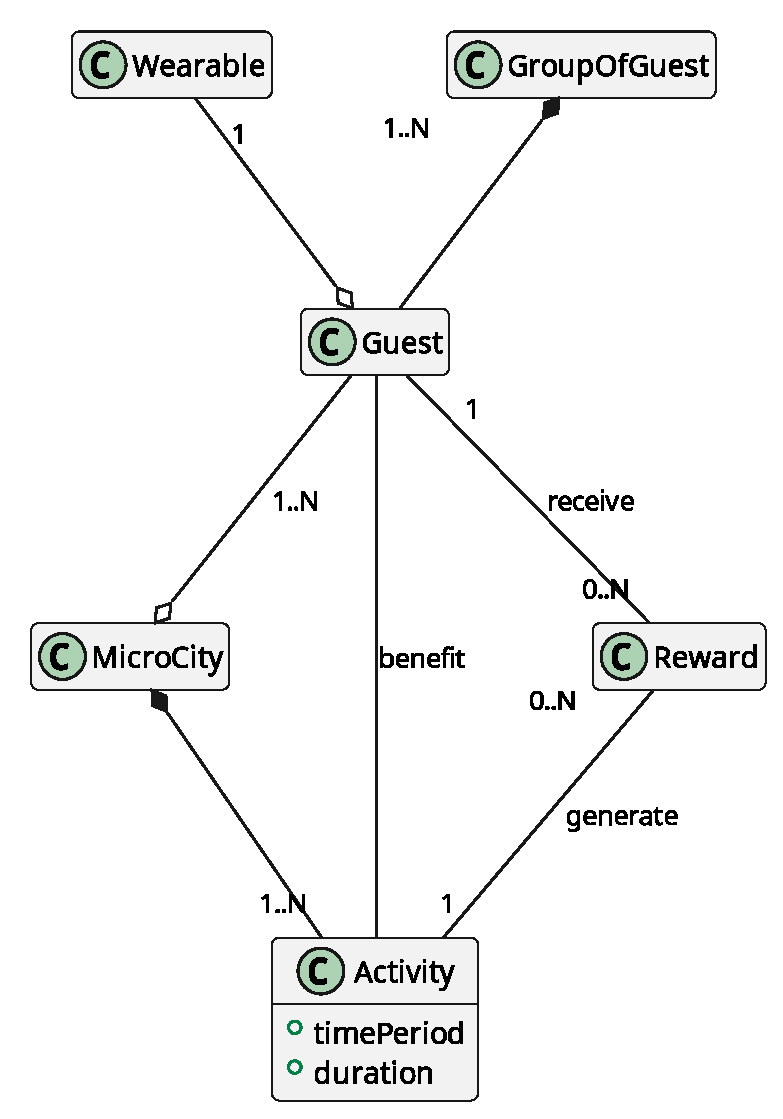
\includegraphics[width=0.55\textwidth]{./img/domain_overview-0}
	\caption{Class diagram of the \textit{Micro City}'s domain model.}
	\label{fig:domain-overview}
\end{figure}

\newpage

The figure \ref{fig:micro-city} shows a diagram representing the organization of a \textit{Micro City}.
A \textit{Micro City} has a map and many workers.
Both activities and the \textit{Micro City} itself may require the payment of a fee, that is an amount of money needed in order to access them.
There are two types of activities: services, that are continuously available during the \textit{Micro City}'s lifetime, and events, that take place in a specific moment and have a limited duration.
Queues may form because of the waiting time needed before a guest can benefit from an activity.

\begin{figure}[H]
	\centering
	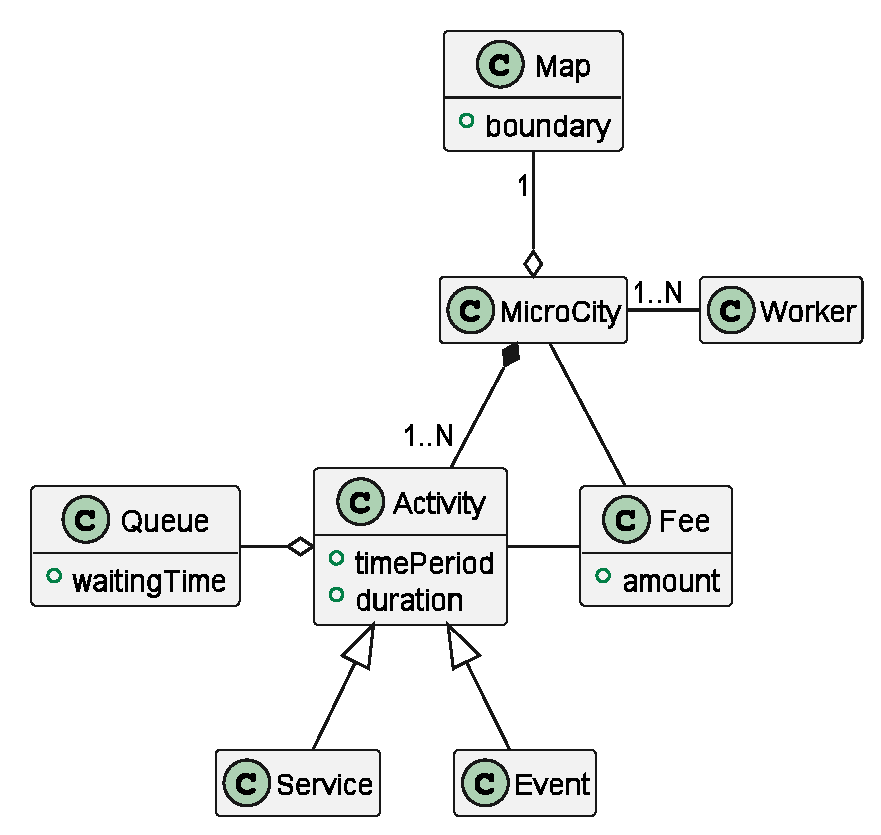
\includegraphics[width=0.7\textwidth]{img/micro_city-0.eps}
	\caption{Class diagram that models the organization of a \textit{Micro City}.}
	\label{fig:micro-city}
\end{figure}

\newpage

The figure \ref{fig:reward} shows the sequence diagram that explains how a guest can obtain a reward.

\begin{figure}[H]
	\centering
	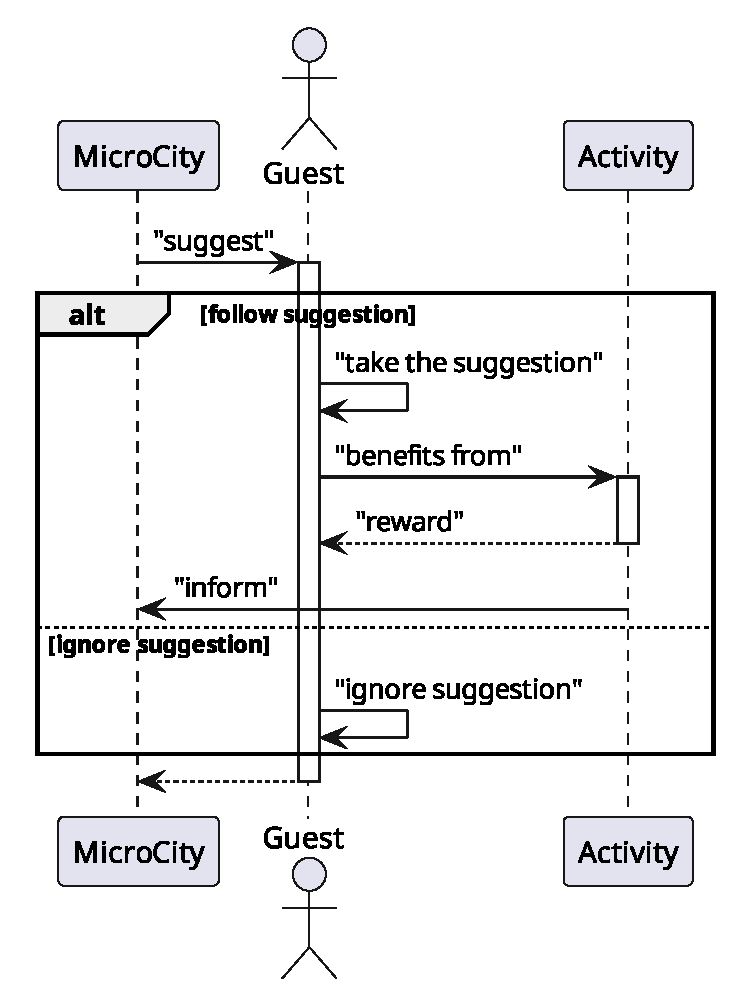
\includegraphics[width=0.6\textwidth]{./img/reward-0}
	\caption{Sequence diagram that shows how to obtain a reward.}
	\label{fig:reward}
\end{figure}

\newpage